In this case, 
\begin{align}
	\vec{V} &= \myvec{ 0 & 0 \\ 0 & 1} \\
	\vec{u} &= \myvec{-2 \\ 0} \\
	f &= 0
\end{align}
For the given line $y=3$, the parameters are
\begin{align}
	\vec{h} = \myvec{0 \\ 3} , \vec{m} = \myvec{1 \\ 0 }
\end{align}
The intersection of 
the line with the conic is obtained from \eqref{eq:tangent_roots} 
as
\begin{align}
	\kappa  = \frac{9}{4} 
\end{align}
The point of contact is given as
\begin{align}
	\vec{a}_0 = \myvec{\frac{9}{4}  \\[1pt] \\ 3}
\end{align}
From \figref{fig:chapters/12/8/1/13/Fig1},
the desired area of the region is obtaioned as
\begin{align}
	\int_{0}^{3} \ \frac{y^2}{4} \,dy &= \frac{1}{12}\sbrak{y^3}_{0}^{3} \\
	&= \frac{1}{12}\brak{27-0} \\
	&= \frac{9}{4} \text{ sq.units}
\end{align}
\begin{figure}[H]
	\begin{center}
		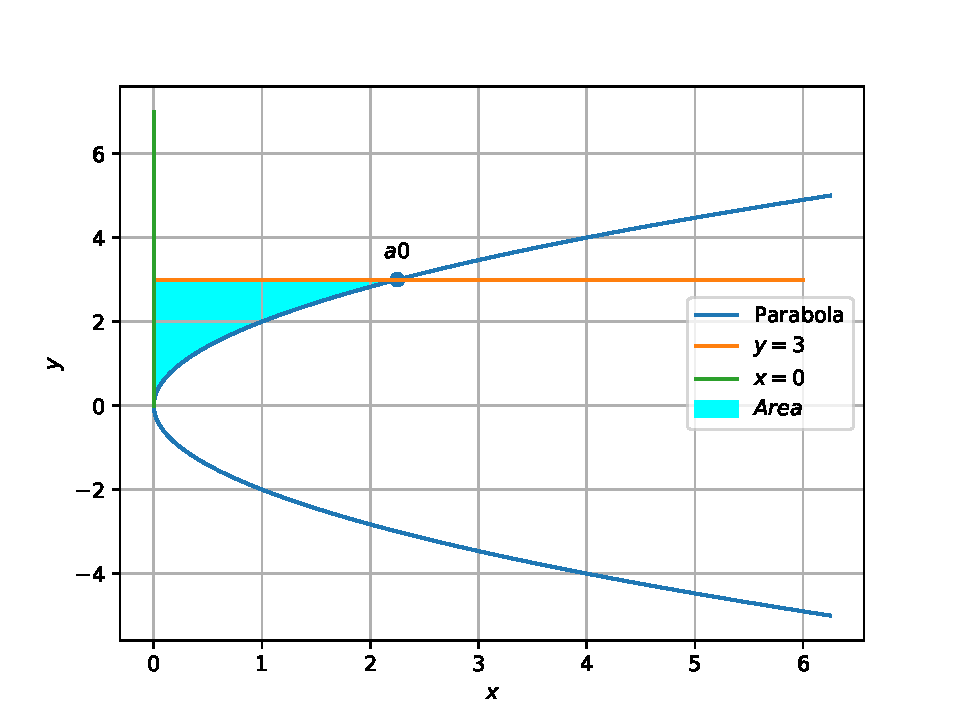
\includegraphics[width=0.75\columnwidth]{chapters/12/8/1/13/figs/problem13.pdf}
	\end{center}
\caption{}
\label{fig:chapters/12/8/1/13/Fig1}
\end{figure}
